\chapter{Introduction}\label{Introduction}
%%%%%%%%%%%%%%%%%%%%%%
% Was wurde untersucht? Was ist daran neu?
% Warum ist das schwierig? Was sind die Herausforderungen?
% Warum relevant?
% Was leistet meine Arbeit? Welche wiss. Beiträge leiste ich?
% Was gibt es für ähnliche Arbeiten? Wie ist meine Anders?
% Der Fahrplan: Wie ist die Arbeit aufgebaut?
%%%%%%%%%%%%%%%%%%%%%%

%    What is the problem?
%    Why is it interesting and important?

\paragraph*{Motivation} Recursion is concise and easy to understand and write, since it resembles our inductive way of thinking about recursive tasks. We start from a nonrecursive basecase and then construct the recursive cases. Evaluation happens by stacking up recursive calls until a basecase is reached and the callstack can be evaluated.

The problem with recursion in general is that it comes with a large overhead. Each call that waits on the result of other function calls is "paused" and the state of execution is pushed to the callstack. This is very expensive in terms of time and memory. All variables, returning addresses etc. need to be copied to the stack when switching the context, and restored when popping the layer. For SQL-UDFs, each call comes with especially large overhead because the UDF-body of every function is planned and the plan needs to be saved until the call returns. Therefore, recursive procedures in SQL are very slow and the limited stack size is quickly exceeded.

%    Why is it hard? (E.g., why do naive approaches fail?)
Iterative solutions with dynamic programming are usually the way to go where recursion is impractical. By iteratively manipulating variables inside the heap memory, overhead from the recursion can be avoided. Additionally, computation is not restricted by stack depth (megabytes) but by heap sizes (gigbytes).

Dynamic Programming \cite{DP_Bellman} aims to avoid redundant recursive calls by saving results of subproblems in a table. Translating a declarative but inefficient algorithm into an imperative language like Java and implementing dynamic programming can be challenging. If you can exploit specific mathematical properties of the problem to constraint the search space, you may come up with a very efficient solution.

In practice, the effort to come up with an near optimal solution is not worth all the effort when a "good enough"-solution would also fit the use-case. Furthermore, the maintainability and portability of a short and simple, declarative piece of code is much higher than the optimized version, that exploits subtle properties of the problem, the database-system or uses other nifty tweaks.

If your target language is not an imperative language but a declarative SQL-query, implementation is less straight forward. You will additionally need a decent amount of knowledge of SQL, the query planner and probably other internals of the database system to avoid all the pitfalls that can slow down your query. Additionally, you sacrifice much readability for performance, obfuscating the logical level with implementation details. This makes the query less maintainable and more error prone.

%    Why hasn't it been solved before? (Or, what's wrong with previous proposed solutions? How does mine differ?)
Our approach fully automatizes the optimization process so that the programmer can keep maintaining a truly declarative UDF in a functional style without concerns of performance. The recursive UDF is automatically translated into an optimized formulation implementing Memoization. The translation is based on slicing the original function into its different evaluation scenarios. The callsite-arguments of the current scenario are evaluated independently from the surrounding context, creating the callgraph. The callgraph is then level-wise evaluated.

\paragraph*{Example}

% fib example
As example, let us comprehend how the Fibonacci function is translated. It is defined as $F_n = F_{n-1} + F_{n-2}$ with $F_0 = 0$ and $F_1 = 1$ \cite[p. 79]{TAOCP_Knuth}. For this example we will use the (slightly awkward) formulation from figure \autoref{intro_fib}.

\begin{figure}[h]\small
    \begin{minipage}[b]{.47\linewidth}
        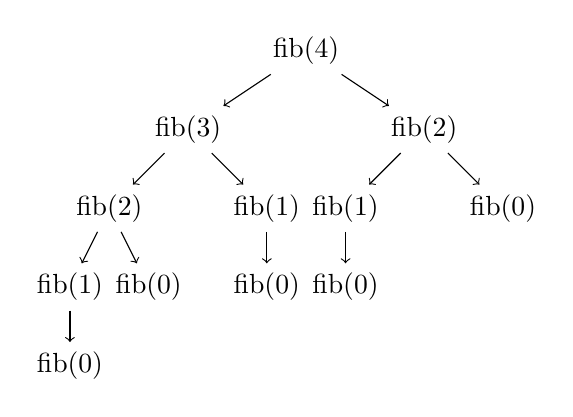
\begin{tikzpicture}
% nodes
\node (n1)     at (2.5, 2) {fib(4)};
    \node (n1-1)   at (1, 1) {fib(3)};
        \node (n1-1-1) at (0, 0) {fib(2)};
            \node (n1-1-1-1) at (-0.5, -1) {fib(1)};
                \node (n1-1-1-1-0) at (-0.5, -2) {fib(0)};
            \node (n1-1-1-2) at (0.5, -1) {fib(0)};
        \node (n1-1-2) at (2, 0) {fib(1)};
            \node (n1-1-2-0) at (2, -1) {fib(0)};
    \node (n1-2)   at (4, 1) {fib(2)};
        \node (n1-2-1) at (3, 0) {fib(1)};
            \node (n1-2-1-0) at (3, -1) {fib(0)};
        \node (n1-2-2) at (5, 0) {fib(0)};
% arrows
\draw[->] (n1)     -- (n1-1);
\draw[->] (n1)     -- (n1-2);
\draw[->] (n1-1)   -- (n1-1-1);
\draw[->] (n1-1)   -- (n1-1-2);
\draw[->] (n1-2)   -- (n1-2-1);
\draw[->] (n1-2)   -- (n1-2-2);
\draw[->] (n1-1-1) -- (n1-1-1-1);
\draw[->] (n1-1-1) -- (n1-1-1-2);
\draw[->] (n1-1-1-1) -- (n1-1-1-1-0);
\draw[->] (n1-1-2) -- (n1-1-2-0);
\draw[->] (n1-2-1) -- (n1-2-1-0);
\end{tikzpicture}
        \caption{Callstack-growth of \texttt{fib(4)}}
        \label{fib_4_callstack}
    \end{minipage}\hfill
    \begin{minipage}[b]{.5\linewidth}
    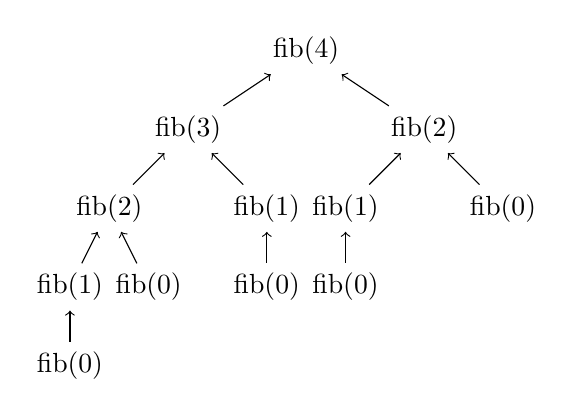
\begin{tikzpicture}
% nodes
\node (n1)     at (2.5, 2) {fib(4)};
    \node (n1-1)   at (1, 1) {fib(3)};
        \node (n1-1-1) at (0, 0) {fib(2)};
            \node (n1-1-1-1) at (-0.5, -1) {fib(1)};
                \node (n1-1-1-1-0) at (-0.5, -2) {fib(0)};
            \node (n1-1-1-2) at (0.5, -1) {fib(0)};
        \node (n1-1-2) at (2, 0) {fib(1)};
            \node (n1-1-2-0) at (2, -1) {fib(0)};
    \node (n1-2)   at (4, 1) {fib(2)};
        \node (n1-2-1) at (3, 0) {fib(1)};
            \node (n1-2-1-0) at (3, -1) {fib(0)};
        \node (n1-2-2) at (5, 0) {fib(0)};
% arrows
\draw[<-] (n1)     -- (n1-1);
\draw[<-] (n1)     -- (n1-2);
\draw[<-] (n1-1)   -- (n1-1-1);
\draw[<-] (n1-1)   -- (n1-1-2);
\draw[<-] (n1-2)   -- (n1-2-1);
\draw[<-] (n1-2)   -- (n1-2-2);
\draw[<-] (n1-1-1) -- (n1-1-1-1);
\draw[<-] (n1-1-1) -- (n1-1-1-2);
\draw[<-] (n1-1-1-1) -- (n1-1-1-1-0);
\draw[<-] (n1-1-2) -- (n1-1-2-0);
\draw[<-] (n1-2-1) -- (n1-2-1-0);
\end{tikzpicture}
        \caption{Callstack-evaluation of \texttt{fib(4)}}
        \label{fib_4_callstack_evaluation}
    \end{minipage}
\end{figure}

% Recursive evaluation in SQL
What happens if we call \mintinline{postgresql}{SELECT fib(4)}? The planner takes some time to have a close look at the query inside \texttt{fib} to consider all possible plans and then executes the cheapest plan. During execution, a number of subcalls occurs that need to be executed before the surrounding query can be evaluated, the calls stack up as illustrated in \autoref{fib_4_callstack}. As soon as a node has the result of all of its children, the node can itself return a result. The leaves of the tree can therefore return a result immediately and the evaluation starts bottom-up (\autoref{fib_4_callstack_evaluation}). 


\begin{figure}[h!]
    \begin{minipage}[b]{.45\linewidth}
    \centering\large
    \sqlcode{snippets/fib_wide.sql}
    \vspace{8mm}
    \subcaption{SQL UDF returning the nth Fibonacci number}
    \label{intro_fib}
    \end{minipage}\hfill
    \begin{minipage}[b]{.45\linewidth}
    \centering\small
    \vspace{-8mm}
    
    \begin{align*}
\Big(&\big\{&\big\langle~&\text{pred}:     &\mintinline{postgresql}{SELECT ($1 = 0)}                  &\\
    &      &    ,~      &\text{query}:    &\mintinline{postgresql}{SELECT 0}                          & \big\rangle \big\}\\
, ~ &\big\{&\big\langle~&\text{pred}:     &\mintinline{postgresql}{SELECT (NOT $1 = 0) AND ($1 = 1)}&\\
    &      &    ,~      &\text{query}:    &\mintinline{postgresql}{SELECT 1 + fib(0)}&    \\
    &      &    ,~      &\text{callsites}:&\langle \text{id}: 1,~\text{args}: (\mintinline{postgresql}{SELECT 0})\big\rangle & \big\rangle\\
    &      &\big\langle~&\text{pred}:     &\mintinline{postgresql}{SELECT (NOT $1 = 0) AND (NOT $1 = 1)}&\\
    &      &    ,~      &\text{query}:    &\mintinline{postgresql}{SELECT fib($1 - 1) + fib($1 - 2)}&\\
    &      &    ,~      &\text{callsites}:&\langle \text{id}: 2,~\text{args}: (\mintinline{postgresql}{SELECT $1 - 1})\rangle &,\\
    &      &            &                 &\langle \text{id}: 3,~\text{args}: (\mintinline{postgresql}{SELECT $1 - 2})\rangle & \big\rangle\big\} \Big)
    \end{align*}
    \subcaption{Recursive scenarios}\label{fib_rec_scenarios}
    \end{minipage}
    \caption{Output of scenario analysis of \mintinline{postgresql}{fib(int)} from \autoref{intro_fib}}\label{fib_analysis_output}
\end{figure}


\begin{figure}[h]
\centering
\begin{tabular}{@{}|c|c|c|@{}}
  \tabname{2}{\strut\texttt{\,callgraph\,}} \\
  \colhd{in\_1} & \colhd{callsite\_id} & \colhd{out\_in} \\
  4 &  2 & 3 \\
  4 &  3 & 2 \\\hline
  3 &  2 & 2 \\
  3 &  3 & 1 \\
  2 &  2 & 1 \\
  2 &  3 & 0 \\\hline
  1 &  1 & 0 \\
  \hline
\end{tabular}
\caption{}\label{tbl:callgraph}
\end{figure}

% Callgraph creation
The idea behind the translation is to simulate this two phases: top-down callstack-growth and bottom-up evaluation. The callstack is created by evaluating only the parts of the UDF that are necessary to observe subsequent recursive calls. First, this are the predicates of the \texttt{CASE}-expression. They are required to detect which callsites are actually called with the given UDF-arguments. Second, the arguments of these callsites need to be evaluated to find out the input-arguments for the subsequent calls. This way, the callstack is built until all callsites lead to basecases. By collecting only unique rows, it is actually not a callstack but a \textit{callgraph} that we create as it contains no duplicate calls.



%To generate the callstack we need to keep track of subsequent calls. To achieve this, we slice the UDF into all possible evaluation scenarios together with predicates to test if a scenario is executed with the current arguments. Now, we can evaluate the \textit{arguments} of the callsites of the current scenario and add subseqent calls to the callstack by this. Substituting the original call arguments (eg. \texttt{\$1} or \texttt{n}) with a reference to the newly discovered arguments from the previous iteration, we are able to generate a complete callstack.

\begin{wrapfigure}{l}{0.35\linewidth}
\centering
\begin{tabular}{@{}|c|c|@{}}
  \tabname{2}{\strut\texttt{\,evaluation\,}} \\
  \colhd{in\_1} & \colhd{result} \\
  0 & 0 \\
  1 & 1 \\
  2 & 1 \\
  3 & 2 \\
  4 & 3 \\
  \hline
\end{tabular}
\caption{}\label{tbl:evaluation}
\end{wrapfigure}

% Callgraph evaluation
Evaluation starts from the bottom: The leaves of the the callstack, ie. the basecases, do not contain any callsites and can therefore evaluated directly and saved. From here evaluation ascends the callstack again and callsites are replaced with references to their results. As soon as all callsites of a scenario have results available, the scenario can be evaluated. This continues until the entire callstack is evaluated and the final result can be returned.


%The idea of the callstack CTE is to collect in every step the arguments of the newly occuring recursive calls. With the data of the analysis, this is a simple task. The following pseudocode gives you an intuition: \mintinline{postgresql}{SELECT in_args, callsite.id, callsite.args FROM scenario.pred p WHERE p.v}. This snippet returns the arguments of a callsite within a scenario that is called with the given \texttt{in\_args} if the predicate of the scenario evaluates to true. If we do this for every callsite in every scenario, we receive a complete level in the tree of the callstack (see \autoref{discovery_strucutre}). To compute the complete callstack, we need to iterate over every set of arguments from the previous call (ie. the level above) and continue collecting calls until no new calls are outputed since we reached the basecases. See \autoref{callstack_recurse} for an illustration.

%By collecting all calls in a table it is also trivial to remove duplicate calls from the callstack before evaluation (figure z), which gives us memoization which speeds up the translation significantly. The callstack table is just a relational representation of the callstack with memoization (Table T).

The output function is generated by filling out a query-template. The data to be filled in is an intermediate representation of the input UDF (\autoref{}), which is generated by a syntax driven analysis of the UDF (\autoref{chapter:analysis}). Its main part is the \textit{scenario analysis} which "slices" the UDF into its different evaluation scenarios. Each scenario consists of a predicate and a query that is semantically equivalent to the original function if the predicate is fulfilled. From the different scenarios the intermediate representation is created. Additional, special properties of the UDF (eg. tail recursion) are detected to choose the best template.

\iffalse
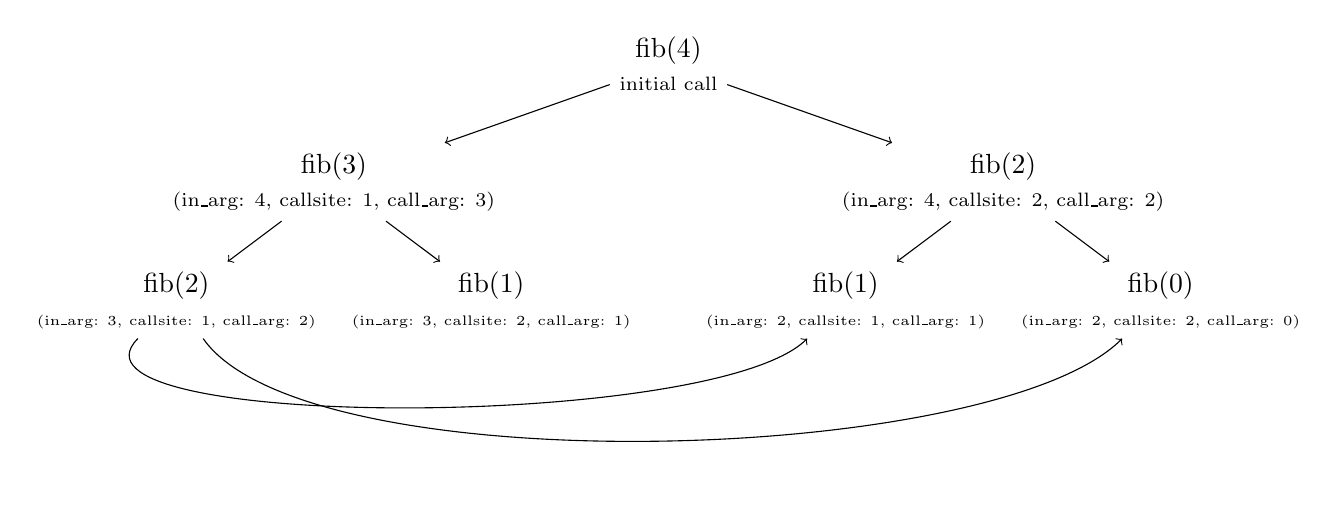
\begin{tikzpicture}[->, level distance=15mm, align=center]
\tikzstyle{level 1}=[sibling distance=85mm]
\tikzstyle{level 2}=[sibling distance=40mm]
\tikzstyle{level 3}=[sibling distance=40mm]
\node{fib(4)\\\scriptsize{initial call}}
  child { node {fib(3)\\\scriptsize{(in\_arg: 4, callsite: 1, call\_arg: 3)}}
    child {node (fib2) {fib(2)\\\tiny{(in\_arg: 3, callsite: 1, call\_arg: 2)}}
      %child {node {fib(1)\\\tiny{(in\_arg: 4, callsite: 2, call\_arg: 2)}} }
      %child {node {fib(0)\\\tiny{(in\_arg: 4, callsite: 2, call\_arg: 2)}} }
    }
    child {node (fib1) {fib(1)\\\tiny{(in\_arg: 3, callsite: 2, call\_arg: 1)}} }
  }
  child {node {fib(2)\\\scriptsize{(in\_arg: 4, callsite: 2, call\_arg: 2)}}
    child {node (fib1) {fib(1)\\\tiny{(in\_arg: 2, callsite: 1, call\_arg: 1)}} }
    child {node (fib0) {fib(0)\\\tiny{(in\_arg: 2, callsite: 2, call\_arg: 0)}} }
  };
\draw[->, bend left=10, out=225, in=225, looseness=0.5] (fib2) edge (fib1);
\draw[->, bend right=5, out=305, in=225, looseness=0.5] (fib2) edge (fib0);
\end{tikzpicture}
\fi

%Based on the recursive scenarios, all callsites are enumerated and their arguments extracted to self-contained queries. The recursive cases are enriched with a list of callsites they contain to check later on whether a result for all callsites of an recursive scenario is present yet.
% Callsite 1: (Argument 1: SELECT \$1 - 1); Callsite 2: (Argument 1: SELECT \$1 - 2)
  
%Now we have all the data required to construct a query that assembles the callgraph. This is achieved by recursivly collecting the arguments of the callsites of those scenarios that occur under the given input argeters. In the beginning, the original input argeters of the function are used. As we recurse, we iterate through the newly added callsite arguments to collect data of further calls. We end up by a relational encoding of a callgraph.

%\sqlcode{snippets/fib_discovery.sql}

%, tracking calls down to the basecases (ie. the nonrecursive scenarios) without evaluating anything from the original function except the callsite-arguments. After the creation of the callgraph, we know the input argeters for the basecases and can evaluate them. With the results of the basecases at hand, it is now possible to continue evaluation up the callgraph. For each recursive scenario we check if for all contained callsites with the given input arguments, a result already exists. If so, the call in the recursive scenario is replaced with the reference to the result and the recursive scenario can be evaluated.

% What are the key components of my approach and results? Also include any specific limitations. 
%The translation of an UDF is split in two major parts, static analysis and template expansion. During static analysis the original UDF is split into different evaluation scenarios with a predicate under that this scenario will be evaluated. The analysis result is used to choose and fill appropriate templates to build the translated function.

%\paragraph*{Static analysis}
%Case analysis: 
%Callsite extraction
%Recursion type detection
%Constant argeter detection
%Hashability checks

%This thesis goal is to extend to range of algorithms for which it is easy to write a fairly performing implementation in standard SQL. I provide inference rules to perform a syntax directed analysis of a given SQL UDF that extracts evaluation scenarios alongside with conditions under which each scenario is executed. To analyze the query correclty, it is necessary to track direct and indirect references to callsites while analyzing the query. Callsites are tracked through FROM, subqueries and CTEs and also takes shadowing into account. Extracted scenarios also contain only actually referenced CTEs, deleting unused CTEs that were referenced by other WHEN-branches. The extracted predicates do not contain any callsites so that they can be used to guard the execution of the scenarios. Predicates, Scenarios and Callsite arguments are extracted in a closed form, so that they contain no free variables and can be evaluated independenty from each other. To achieve this, none of these may reference a row-variables from an outside FROM, only table-variables may be referenced, including outside CTEs. This also limits the ability of the UDF to perform meaningful computations that return tabular results, which we forbid entirely for now.

%Each scenario is generated from the different branches of a \CASE-statement and the predicates that need to be fulfilled to reach a given \WHEN-branch. Each resulting scenario is semantically equivalent to the original query if its predicate is fulfilled. All scenarios combined are semantically equivalent to the original query. The scenarios are divided into basecases, that do not contain any recursive callsites, and recursive cases that do contain one or more callsites. Some more analysis is performed on the generated scenarios to detect properties of the function like tail recursion.



%\paragraph*{Template-based translation}
%Callstack
%Basecases
%TerminationCheck
%Evaluation
% From the extracted data an appropriate template is filled, forming the translation. The translation utilizes the iterative nature of WITH RECURSIVE to implement an actual iterative version of the recursive UDF. First, the callstack is discovered by iterativly collecting the new arguments of the callsites in the appropiate scenario. Second, the basecases are evaluated and all new computable results are collected. This repeats until the final result is computed. Cases where the translation would terminate but the original does not are detected and an infinite loop is created to mimic the original behaviour.

% The translation template consists of a discovery-phase and an evaluation-phase. During discovery the callstack is built, collecting all recursive calls down to the nonrecursive basecases. From the discovery-table it is now possible to look up the input arguments that lead to a nonrecursive scenario which can be used to begin the recursive evaluation process. As soon as results for all callsites of a given scenario exist, this scenario can be evaluated. The query continues recursively until the argeter of the original call is found in the evaluation table.
    
\paragraph*{Contributions} The general translation idea has been developed at the Database Systems Research Group at WSI in Tübingen. My main contribution is a first working implementation of this approach in Haskell, targeting PostgreSQL 10.6. I provide a handy command line tool \texttt{twr} to perform translations of UDFs from the database or from a SQL-file. A folder of UDFs or even an entire database can be batch-translated. The translated function(s) can be renamed and saved to file/folder or persisted in the database. Optimizations can selectively be disabled and analysis output can be shown.

Beside a first working implementation, I contributed some improvements to the inference rules to slice the original UDF into its evaluation scenarios. Here, my main contribution is the addition of rules to handle CTEs that may be nested and can contain callsites. Further, I have rewritten the rules for handling case-expressions to work in a step-wise fashion. This allows recursive predicates that contains nested \texttt{CASE}-expressions. The step-wise operation also made implementation easier. I added also a set of simple rules to extract the arguments from callsite while keeping references to used CTEs.

I also contributed a number of improvements to the templates. Most notably, I have rewritten the template for evaluating recursive scenarios that removes array aggregation and thereby allows arbitrary array arguments\footnote{When aggregating arrays, \texttt{array\_agg} requires all arrays to have the same dimensionality. This renders non-constant array arguments impossible.}. Furthermore, I simplified result selection and non-termination by adding the original call to the callgraph. The pattern to stop evaluation of the recursive CTE when no new results are created while adding old results to the result was also created by me.

% There are two interesting parts regarding the translation. The first is the template itself and its various optimizations that can be applied under certain circumstances, eg. when the function is tail recursive. The other interesting part is how to derive the sliced representation of the UDF that is required to fill the templates. I provide a small-step operational semantics over a subset of SQL to compile a query into its scenarios.

% First I will establish the backgrounds required for this thesis. The evaluation of SQL-queries, which is important to understand query performance, is covered first. Special focus is laid on the evaluation of WITH RECURSIVE which we utilize to create a translation from a recursive to an actually iterative function. The evaluation of SQL-UDFs is covered then, showing differences in evaluation that lead to the poor performance of recursive UDFs. Important forms of recursion, as well as pros and cons are dicussed afterwards. The background-chapter closes with a short primer on Small step Operational Semantics.